\documentclass[]{standalone} 
\usepackage[tikz,math,plot]{forsyde}
\usepackage{forsyde-atom-docs}

\begin{document}
\begin{docimage}{inits}
  \begin{tikzpicture}[]
    \trans[transition=v1gv1, type=inits] (a) {};
    \path[v] (a) edge[<-] ++(-2,0) edge[->,token=vector] ++(2,0); 
  \end{tikzpicture}
\end{docimage}

\begin{docimage}{inits-net}
\begin{tikzpicture}[scale = .7]
\vector[] (0,.5) - (0,4.5); \vector[] (2.2,0.5) - (2.2,4.5);
\foreach \i in {1,2,3,4} {
  \vector[shorten >= 1pt, shorten <= 1pt] ($(2,\i)-(0,.5)$) - ($(2,\i)+(0,.5)$);
  \signal[] (-1,\i) -> (0,\i);
  \vector[] (2,\i) -> (3,\i);
  \foreach \j in {1,...,\i} {
    \pgfmathsetmacro{\y}{\j + (\i - \j - (4 - \i) - (4 - \j) + (4 - \j) ) / 16}
    \signal[] (0,\i) -> (2,\y);
  }
}
\end{tikzpicture}
\end{docimage}

\begin{docimage}{tails}
  \begin{tikzpicture}[]
    \trans[transition=v1gv1, type=tails] (a) {};
    \path[v] (a) edge[<-] ++(-2,0) edge[->,token=vector] ++(2,0); 
  \end{tikzpicture}
\end{docimage}

\begin{docimage}{tails-net}
\begin{tikzpicture}[scale = .7]
\vector[] (0,.5) - (0,4.5); \vector[] (2.2,0.5) - (2.2,4.5);
\foreach \i in {1,2,3,4} {
  \vector[shorten >= 1pt, shorten <= 1pt] ($(2,\i)-(0,.5)$) - ($(2,\i)+(0,.5)$);
  \signal[] (-1,\i) -> (0,\i);
  \vector[] (2,\i) -> (3,\i);
  \foreach \j in {\i,...,4} {
    \pgfmathsetmacro{\y}{\j + (2 * \i - 2 * \j + (\j - 1) ) / 16}
    \signal[] (0,\i) -> (2,\y);
  }
}
\end{tikzpicture}
\end{docimage}


\begin{docimage}{reverse}
  \begin{tikzpicture}[]
    \trans[transition, type=reverse] (a) {};
    \path[v] (a) edge[<-] ++(-2,0) edge[->,token=vector] ++(2,0); 
  \end{tikzpicture}
\end{docimage}

\begin{docimage}{reverse-net}
\begin{tikzpicture}[scale = .5]
  \vector[] (0,.5) - (0,6.5); \vector[] (2,0.5) - (2,6.5);
  \foreach \i/\j in {1,...,6} {
    \pgfmathtruncatemacro\j{7-\i}
    \path[s,->]
    (-2,\i) edge (0,\i)
    (0,\i) edge (2,\j)
    (2,\j) edge (4,\j)
    ;
  }
\end{tikzpicture}
\end{docimage}


\begin{docimage}{filteridx}
  \begin{tikzpicture}[]
    \trans[transition, f={$\noexpand\id{odd}$}, type=filterIdx] (a) {};
    \path[v] (a) edge[<-] ++(-2,0) edge[->,token=vector] ++(2,0); 
  \end{tikzpicture}
\end{docimage}

\begin{docimage}{filteridx-net}
\begin{tikzpicture}[scale = .5]
  \vector[] (0,.5) - (0,6.5); \vector[] (2,0.5) - (2,6.5);
  \foreach \i in {1,...,6} {
    \path[s,->] (-2,\i) edge (0,\i) (2,\i) edge (4,\i);
  }
  \foreach \i in {2,4,6} {
    \path[s,->] (0,\i) edge (2,\i);
  }
\end{tikzpicture}
\end{docimage}


\begin{docimage}{replace}
  \begin{tikzpicture}[]
    \trans[transition, ni=2, f={3}, type=replace] (a) {};
    \path[v] (a.w2) edge[<-] ++(-2,0) (a.e1) edge[->,token=vector] ++(2,0);
    \path[s] (a.w1) edge[<-] ++(-2,0);
  \end{tikzpicture}
\end{docimage}

\begin{docimage}{replace-net}
\begin{tikzpicture}[scale = .5]
  \vector[] (0,-.5) - (0,-6.5); \vector[] (2,-0.5) - (2,-6.5);
  \foreach \i in {1,...,6} {
    \path[s,->] (-2,-\i) edge (0,-\i) (2,-\i) edge (4,-\i);
  }
  \foreach \i in {1,2,4,5,6} {
    \path[s,->] (0,-\i) edge (2,-\i);
  }
  \path[s] (0,0) edge (-2,0) edge[->] (2,-3);
\end{tikzpicture}
\end{docimage}


\begin{docimage}{group}
  \begin{tikzpicture}[]
    \trans[transition=v1gv1, f=3, type=group] (a) {};
    \path[v] (a) edge[<-] ++(-2,0) edge[->,token=vector] ++(2,0); 
  \end{tikzpicture}
\end{docimage}

\begin{docimage}{group-net}
\begin{tikzpicture}[scale = .5]
  \vector[] (0,-.5) - (0,-6.5); \vector[] (2.2,-0.5) - (2.2,-6.5);
  \path[v](2,-.5) edge (2,-3.35) (2,-3.65) edge (2,-6.5);
  \foreach \i in {1,...,6} {
    \path[s,->] (-2,-\i) edge (0,-\i);
    \path[s,->] (0,-\i) edge (2,-\i);
  }
  \path[v,->] (2.2,-2.25) edge ++(2,0) (2.2,-4.75) edge ++(2,0);
\end{tikzpicture}
\end{docimage}


\begin{docimage}{shiftr}
  \begin{tikzpicture}[]
    \trans[transition, ni=2, type=shiftr] (a) {};
    \path[v] (a.w1) edge[<-] ++(-2,0) (a.e1) edge[->,token=vector] ++(2,0);
    \path[s] (a.w2) edge[<-] ++(-2,0);
  \end{tikzpicture}
\end{docimage}

\begin{docimage}{shiftr-net}
\begin{tikzpicture}[scale = .5]
  \vector[] (0,-.5) - (0,-6.5); \vector[] (2,-0.5) - (2,-6.5);
  \foreach \i in {1,...,6} {
    \path[s,->] (-2,-\i) edge (0,-\i) (2,-\i) edge (4,-\i);
  }
  \foreach \i in {1,...,5} {
    \pgfmathtruncatemacro{\j}{\i + 1}
    \path[s,->] (0,-\i) edge (2,-\j);
  }
  \path[s] (0,0) edge ++(-2,0) edge[->] (2,-1);
\end{tikzpicture}
\end{docimage}

\begin{docimage}{shiftl}
  \begin{tikzpicture}[]
    \trans[transition, ni=2, type=shiftl] (a) {};
    \path[v] (a.w1) edge[<-] ++(-2,0) (a.e1) edge[->,token=vector] ++(2,0);
    \path[s] (a.w2) edge[<-] ++(-2,0);
  \end{tikzpicture}
\end{docimage}

\begin{docimage}{shiftl-net}
\begin{tikzpicture}[scale = .5]
  \vector[] (0,-.5) - (0,-6.5); \vector[] (2,-0.5) - (2,-6.5);
  \foreach \i in {1,...,6} {
    \path[s,->] (-2,-\i) edge (0,-\i) (2,-\i) edge (4,-\i);
  }
  \foreach \i in {2,...,6} {
    \pgfmathtruncatemacro{\j}{\i - 1}
    \path[s,->] (0,-\i) edge (2,-\j);
  }
  \path[s] (0,-7) edge ++(-2,0) edge[->] (2,-6);
\end{tikzpicture}
\end{docimage}

\begin{docimage}{rotr}
  \begin{tikzpicture}[]
    \trans[transition, ni=2, type=rotr] (a) {};
    \path[v] (a.w1) edge[<-] ++(-2,0) (a.e1) edge[->,token=vector] ++(2,0);
    \path[s] (a.w2) edge[<-] ++(-2,0);
  \end{tikzpicture}
\end{docimage}

\begin{docimage}{rotr-net}
\begin{tikzpicture}[scale = .5]
  \vector[] (0,-.5) - (0,-6.5); \vector[] (2,-0.5) - (2,-6.5);
  \foreach \i in {1,...,6} {
    \path[s,->] (-2,-\i) edge (0,-\i) (2,-\i) edge (4,-\i);
  }
  \foreach \i in {1,...,5} {
    \pgfmathtruncatemacro{\j}{\i + 1}
    \path[s,->] (0,-\i) edge (2,-\j);
  }
  \path[s] (0,-6) edge[->] (2,-1);
\end{tikzpicture}
\end{docimage}


\begin{docimage}{rotl}
  \begin{tikzpicture}[]
    \trans[transition, ni=2, type=rotl] (a) {};
    \path[v] (a.w1) edge[<-] ++(-2,0) (a.e1) edge[->,token=vector] ++(2,0);
    \path[s] (a.w2) edge[<-] ++(-2,0);
  \end{tikzpicture}
\end{docimage}

\begin{docimage}{rotl-net}
\begin{tikzpicture}[scale = .5]
  \vector[] (0,-.5) - (0,-6.5); \vector[] (2,-0.5) - (2,-6.5);
  \foreach \i in {1,...,6} {
    \path[s,->] (-2,-\i) edge (0,-\i) (2,-\i) edge (4,-\i);
  }
  \foreach \i in {2,...,6} {
    \pgfmathtruncatemacro{\j}{\i - 1}
    \path[s,->] (0,-\i) edge (2,-\j);
  }
  \path[s] (0,-1) edge[->] (2,-6);
\end{tikzpicture}
\end{docimage}


\begin{docimage}{gather}
  \begin{tikzpicture}[]
    \trans[transition, f={$\noexpand\SkelVec{2,3,6}$}, type=gather] (a) {};
    \path[v] (a.w1) edge[<-] ++(-2,0) (a.e1) edge[->,token=vector] ++(2,0);
  \end{tikzpicture}
\end{docimage}

\begin{docimage}{gather-net}
\begin{tikzpicture}[scale = .5]
  \vector[] (0,1) - (0,6); \vector[] (2,1) - (2,6);
  \foreach \i in {1,...,6} {
    \signal[] (-1,\i) -> (0,\i);
  }
  \foreach \i in {1,4,5} {
    \signal[] (0,\i) -> (2,\i);
    \signal[] (2,\i) -> (3,\i);
  }
\end{tikzpicture}
\end{docimage}


\begin{docimage}{scatter}
  \begin{tikzpicture}[]
    \trans[transition=v2v1, ni=2, f={$\noexpand\SkelVec{2,3,6}$}, type=scatter] (a) {};
    \path[v] (a.w1) edge[<-] ++(-2,0) (a.w2) edge[<-] ++(-2,0) (a.e1) edge[->,token=vector] ++(2,0);
  \end{tikzpicture}
\end{docimage}

\begin{docimage}{scatter-net}
\begin{tikzpicture}[scale = .5]
  \vector[] (0,.5) - (0,3); \vector[] (2,.5) - (2,3);
  \vector[] (0,0) - (0,-2);
  \foreach \i in {1,...,6} {
    \pgfmathsetmacro{\y}{\i * .5}
    \signal[] (-1,\y) -> (0,\y);
    \signal[] (2,\y) -> (3,\y);
  }
  \foreach \i [count=\n from 0] in {5,4,1} {
    \pgfmathsetmacro{\y}{\i * .5}
    \signal[] (-1,-\n) -> (0,-\n);
    \signal[] (0,-\n) -> (2,\y);
  } 
  \foreach \i in {2,3,6} {
    \pgfmathsetmacro{\y}{\i * .5}
    \signal[] (0,\y) -> (2,\y);
  } 
\end{tikzpicture}
\end{docimage}


\begin{docimage}{bitrev}
  \begin{tikzpicture}[]
    \trans[transition, type=bitrev] (a) {};
    \path[v] (a.w1) edge[<-] ++(-2,0) (a.e1) edge[->,token=vector] ++(2,0);
  \end{tikzpicture}
\end{docimage}

\begin{docimage}{bitrev-net}
\begin{tikzpicture}[scale = .5]
  \vector[] (0,.5) - (0,4); \vector[] (2,.5) - (2,4);
  \foreach \i/\j in {1/8,2/4,3/6,4/2,5/7,6/3,7/5,8/1} {
    \pgfmathsetmacro{\x}{\i / 2}
    \pgfmathsetmacro{\y}{\j / 2}
    \signal[] (-1,\x) -> (0,\x);
    \signal[] (2,\x) -> (3,\x);
    \signal[] (0,\x) -> (2,\y);
  }
\end{tikzpicture}
\end{docimage}

\begin{docimage}{zipx}
  \begin{tikzpicture}
  \trans[transition=s1v1, rotate shape=180, ni=4, no=1, type=zipx](p) <0,0> {};
  \foreach \i in {1,...,4} {
    \signal[token=scalar] ($(p.w\i)-(1,0)$) -> (p.w\i);
  }
  \signal[token=vector] (p.e1) -> ($(p.e1)+(1,0)$);
\end{tikzpicture}
\end{docimage}

\begin{docimage}{unzipx}
  \begin{tikzpicture}
  \trans[transition=s1v1, ni=1, no=4, type=unzipx](p) <0,0> {};
  \foreach \i in {1,...,4} {
    \signal[token=scalar] ($(p.e\i)+(1,0)$) <- (p.e\i);
  }
  \signal[token=vector] (p.w1) <- ($(p.w1)-(1,0)$);
\end{tikzpicture}
\end{docimage}

\end{document}



%%% Local Variables:
%%% TeX-command-default: "Make"
%%% mode: latex
%%% TeX-master: t
%%% End:
